\section{Methodology}
How, then, can \xQ{} be calculated? Following from discussion in the previous section a surrogate model, \surrogate{}, can be learned to predict the reward distribution \rwdstarapprox{} of the trusted reference solver \solvestar{} on task \task{} as shown in Fig.~\ref{fig:sq_train}.

The candidate solver \solve{} must then be evaluated w.r.t. the trusted solver \solvestar{}. This is done by comparing \rwdstarapprox{} (the predicted performance of \solvestar{} on task \task) and \rwd{} (the simulated performance of solver \solve{} on task \task) as illustrated in Fig.~\ref{fig:sq_test}.

Figure \ref{fig:sq_v2} illustrates some of the key quantities involved in calculating \xQ. The basic premise is simple: \emph{find the difference between the trusted solver ($T$) and the candidate solver ($C$) while taking into account which solver has move expected reward, and the overall range of rewards of the trusted solver over many tasks}.

% \begin{figure}[tb]
    % \centering
    % 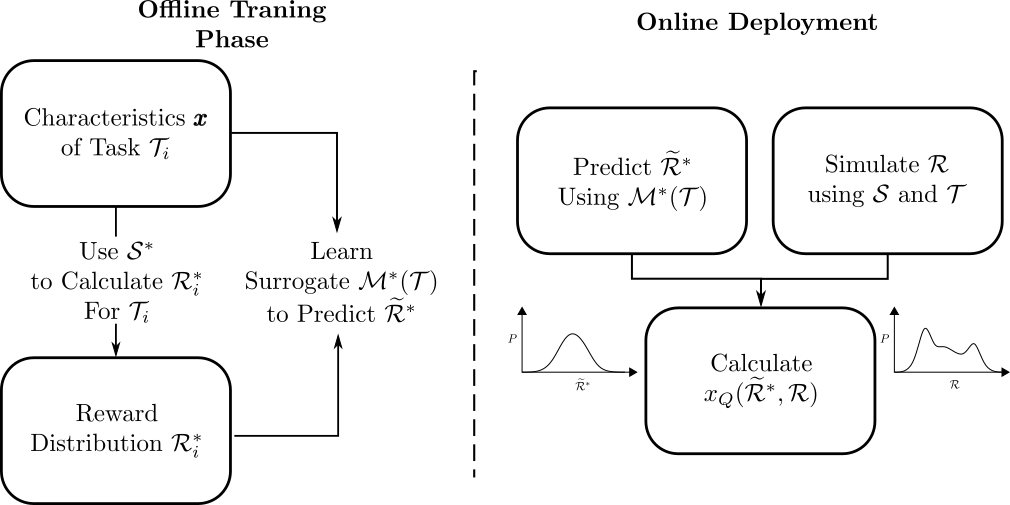
\includegraphics[width=0.95\linewidth]{Figures/SQ_train_test.png}
    % \caption{Depiction of the training phase of the surrogate function \surrogate, and the test, or online deployment, phase where \xQ{} is calculated.}
    % \label{fig:sq_train_test}
% \end{figure}%
\begin{figure}[tbp]
    \centering
    \begin{subfigure}[c]{0.50\linewidth}
        \centering
        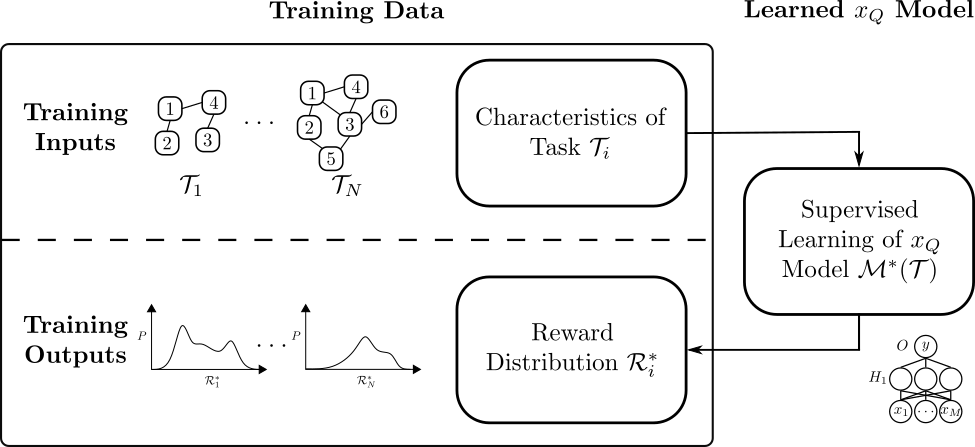
\includegraphics[width=0.8\linewidth]{Figures/SQ_train.png}
        \vfill
        \caption{Offline Training}
        \label{fig:sq_train}
    \end{subfigure}%
    \hfill
    \begin{subfigure}[c]{0.50\linewidth}
        \centering
        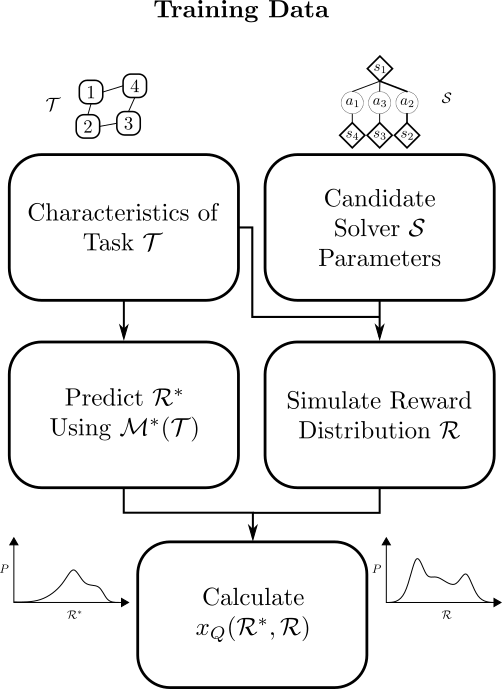
\includegraphics[width=0.8\linewidth]{Figures/SQ_test.png}
        \caption{Online Deployment}
        \label{fig:sq_test}
    \end{subfigure} 
    \caption{Depiction of the training phase of the surrogate function \surrogate, and the test, or online deployment, phase where \xQ{} is calculated.}
    \label{fig:sq_test_train}
\end{figure}

\subsection{Learning \surrogate}
The surrogate model \surrogate{} can be any model capable of predicting \rwdstarapprox{} given \task. In the formulation presented above \rwdstariapprox{} only represents the mean and standard deviation for \rwdstari{} (this makes the learning problem less complicated, but is not necessary). Figure \ref{fig:sq_train} depicts how the surrogate model is trained. Learning \surrogate{} would typically be done `offline' when more computation power and time are available.

\subsection{Calculating \xQ}
In order to compare two solvers the resultant reward distributions that each of those solvers produce are compared (as stated in Sec.~\ref{sec:compare_policies}). If two solvers produce an identical reward distribution \emph{for a given task}, then they can be considered equal in their `quality', or considered equally `capable'. Conversely, if the two distributions are very different (for the same task) then their quality, or capability, is also different. Following, the detailed components of the \xQ{} formulation are discussed, refer to Fig.~\ref{fig:sq_v2} for a visual 

\subsubsection{Hellinger Metric $\bm{H^2}$} \label{sec:hellinger}
Perhaps the easiest way of calculating the similarity between distributions is to find the `distance' between them. The Hellinger metric (\hell) is such a measure, and is \emph{bounded} between 0 and 1, where 0 means the distributions are identical. The maximum distance, 1, is achieved when distribution $P$ assigns zero probability at every point in which distribution $Q$ assigns probability.  \hell{} has different forms based on the type of analytical distributions being compared. For the purposes of calculating \xQ{} the from for two distributions ($P \sim (\mu_1,\sigma_1), Q\sim(\mu_2,\sigma_2)$) is useful:
\begin{align}
    H^{2}(P,Q) = 1-\sqrt{\frac{2\sigma_P\sigma_Q}{\sigma_P^2+\sigma_Q^2}}\exp{\left(-\frac{1}{4}\frac{(\mu_P-\mu_Q)^2}{\sigma_P^2+\sigma_Q^2}\right)}
\end{align}

To aid in forming intuition, see Fig.~\ref{fig:hellinger_surf} which shows how the distance measure varies with a changing $\mu_1$ and $\sigma_1$. In this example $\mu_2=0.0$ and $\sigma_2=1.0$.

Using \hell{} the overlap between $T$ and $C$ can be calculated. However, there are a couple of other considerations that need to be taken into account. 

\subsubsection{Difference in Expected Reward: $\bm{\Delta \mu}$}
\hell{} as a distance measure is always greater than zero, and so information that indicates if a distribution is generally better or worse (i.e. more or less expected reward) is lost. In order to keep this information the sign of the difference between the expected rewards of the two distributions $\text{sgn}(\mu_1-\mu_2)$ can be used.

\subsubsection{Relative Difference on a Global Scale: $\bm{(r_H-r_L)}$}
The next consideration is that just because distance between two distributions may be great or small, does not mean the same applies from a higher-level, or global, perspective. In an extreme case one might imagine two Normal distributions with means $\mu_1=1$ and $\mu_2=2$, and low variances $\sigma_1^2=\sigma_2^2=1e\-5$. In this case the Hellinger distance between the two would be $1$ since they share practically no overlapping probability. However, if the means of the distributions are nearly equal on the global scale (e.g. rewards from many other tasks are on the range $[-1e3,1e3]$), then the quantity of \hell{} isn't critical from that perspective.

\subsubsection{Putting the pieces together}
Using the points discussed above the expression for the quality of candidate solver \solve{} w.r.t. the reference solver \solvestar{} is (again see Fig.~\ref{fig:sq_v2} for intuition):
\begin{align}
    \text{q} &= \text{sgn}(\Delta \mu)f^{\alpha}\sqrt{H^{2}(T,C)} \label{eq:q}
\end{align}

Where $\Delta \mu = \mu_c-\mu_t$, and $f = \Delta \mu/(r_H-r_L)$. The exponent $\alpha$ is a parameter that affects the influence that $f$ has with respect to \hell. In essence, should the relationship of the effects of $f$ and \hell{} be $1:1$? In practice $\alpha=1$ does not yield desirable results. \hell{} should be more influential on $\text{q}$ as $f$ grows smaller, and $f$ should be more influential as it increases. We have found $\alpha=1/2$ gives results that `make sense'; future work could investigate the `best' value for $\alpha$ via user studies.

As formulated the only requirement of reward distributions T and C is that they have a known mean and standard deviation. In essence \xQ{} is a measure of the distance of two arbitrary distributions using only their first two moments.

\subsubsection{Accommodations For Humans}
While \hell{} is on the domain $[0,1]$, the quantity $f$ from Eq. \ref{eq:f} is $[0,\infty]$. Because of this it is desirable to use a `squashing function' to keep \xQ{} value within some range and avoid arbitrarily large values that can be confusing to humans. The general logistic equation is useful for this.
We use $L=2$ so that when $s=0$ (distributions are identical) \xQ{} will be 1. The parameter $k$ is selected to be $5$ so that \xQ{} `saturates' at around $\text{q}=\pm1$.
\begin{align}
    x_{Q} &= \frac{2}{1+exp(-\text{q}/5)}\label{eq:SQ}
\end{align}

\subsection{Examples}
A toy example is useful in evaluating whether \xQ{} yields desirable results. Figure~\ref{fig:sq_thry1} illustrates a toy example showing the expected reward (with uncertainty) for a trusted solver \solvestar{} given a specific, generic, task parameter, as well as that of a `candidate' solver \solve. Different points of interest (indicating specific values of the task parameter) are highlighted by a star. The table on the side shows the values of \xQ{} calculated for different cases.

At B the candidate solver has a lower expected reward than the trusted solver and a higher variance than the trusted solver. Intuitively \xQ{} should be less than one. As shown when $r=5$ (i.e. $r_H-r_L=5$, the global reward range is `large') $x_Q=0.667$ which indicates that the candidate solver is marginally less capable than the trusted solver, and when $r=0.05$ then $x_Q=0.002$ indicates that \solve{} is much less capable than \solvestar.

At C the candidate solver \solve{} has higher expected reward than \solvestar, but a larger variance. Intuitively we would expect \xQ{} of \solve{} to be a little greater than one, and in fact when $r=5$, $x_Q=1.095$. As the global reward range $r$ decreases the difference in capability between \solve{} and \solvestar{} increases with $x_Q=1.995$ at $r=0.005$. These calculations indicate that \xQ{} performs as expected. In Sec.~\ref{sec:results} a more realistic scenario is considered. 

\begin{figure}[tbp]
    \centering
    \begin{subfigure}[c]{0.65\linewidth}
        \centering
        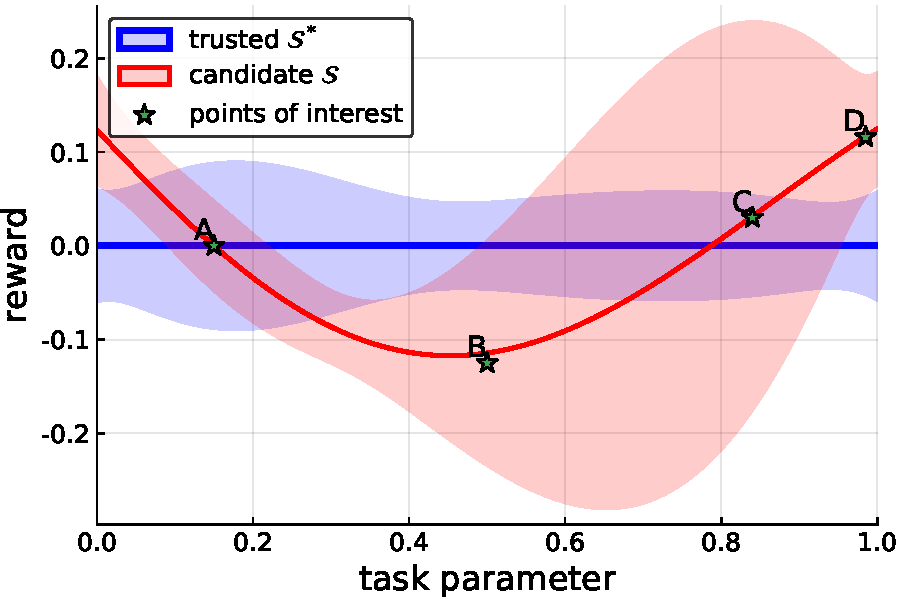
\includegraphics[width=1.0\linewidth]{Figures/p1.pdf}
        \vfill
        % \caption{tst}
        % \label{fig:}
    \end{subfigure}%
    \hfill
    \begin{subfigure}[t]{0.35\linewidth}
        \centering
        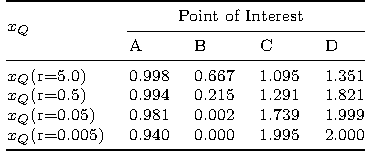
\includegraphics[width=1.0\linewidth]{Figures/p1_table.pdf}
        % \caption{Candidate solver depth 1}
        % \label{fig:med_roadnet}
    \end{subfigure} 
    \caption{Assessing \xQ{} calculation on reward fxn's: \solvestar{} (blue) and \solve{} (red). Points of interest indicated by a star.}
    \label{fig:sq_thry1}
\end{figure}
